\chapter{Results}
\label{ch:results}

In this chapter, the results of the analysis are presented. First I present the results of the
efficiency analysis in \autoref{sec:efficiency_angres}. The results are based on a dataset consisting of
20 runs. Furthermore, I present the results of the angular resolution for a combined metric with the efficiency.
Then, in \autoref{sec:metrics}, the metrics of each resulting combination of hyperparameters
are presented. In \autoref{sec:performance}, the performance of each cleaning algorithm compared
to the default settings is presented. Finally, a comparison of the different cleaning algorithms is
presented in \autoref{sec:comparison}.


\section{Analysis of Efficiency and Angular Resolution}
\label{sec:efficiency_angres}

To determine the optimal hyperparameters, I first analyzed the efficiency of the different cleaning algorithms.
The efficiency is determined by the number of events that are reconstructed after cleaning. For this work
I chose \(\num{20}\) intervals within \(\num{0}\) and \(\num{1}\) with a step size of \(\num{0.05}\).
For each interval those datasets are selected, where the efficiency lies between the lower and upper
bound of the interval. Then the minimum angular resolution is determined for each interval. The parameters
of these datasets are then selected to be the optimal parameters for each cleaning algorithm. This not
only allows for a comparison of the cleaners but also a decision on a trade-off between the efficiency
and the angular resolution, namely having a better angular resolution, but a lower efficiency or
a higher efficiency but a higher and therefore worse angular resolution.
The results for the efficiency are listed in \todo{complete table}\autoref{tab:efficiency} and the results for the angular
resolution in \todo{complete table}\autoref{tab:angres}.

\begin{table}
    \centering
    \caption{The results of the analysis for the efficiency of each cleaning algorithm. The efficiency
    is calculated as the ratio of the number of reconstructed events $n_{\mathrm{reco}}$ and the number
    of total events $n_{\mathrm{total}}$. The table lists the lower and upper limits of each efficiency
    interval. The efficiency is then calculated as the mean over the whole energy range of the dataset.
    The listed efficiencies are the ones where the mean angular resolution is minimal for the given
    interval.}
    \label{tab:efficiency}
    \rowcolors{0}{white!92!black}{}
    \begin{tabular}{r r r r r r}
        \hiderowcolors
        & & \multicolumn{4}{c}{Mean Efficiency} \\
        {$\eff_{\mathrm{lower}}$} & {$\eff_{\mathrm{upper}}$} & {\texttt{tailcuts}} & {\texttt{mars}} & {\texttt{fact}} & {\texttt{tcc}} \\
        \addlinespace[0.5em]
        \showrowcolors
        \input{build/efficiency.txt}
    \end{tabular}
\end{table}

\begin{table}
    \centering
    \caption{Angres}
    \label{tab:angres}
    \rowcolors{0}{white!92!black}{}
    \begin{tabular}{r r r r r r}
        \hiderowcolors
        & & \multicolumn{4}{c}{Mean Angular Resolution} \\
        {$\eff_{\mathrm{lower}}$} & {$\eff_{\mathrm{upper}}$} & {\texttt{tailcuts}} & {\texttt{mars}} & {\texttt{fact}} & {\texttt{tcc}} \\
        \addlinespace[0.5em]
        \showrowcolors
        \input{build/angular_resolution.txt}
    \end{tabular}
\end{table}
From the tables, one can see that there is a clear trade-off in choosing between efficiency and angular resolution.
As such, for further comparison of the cleaning algorithms, the corresponding datasets for the efficiency and
the angular resolution are plotted in \autoref{fig:efficiency_angres} for the intervals
\([\num{0.25}, \num{0.30}]\) and \([\num{0.45}, \num{0.50}]\) \todo{explain decision of displaying these}.

\begin{figure}
    \centering
    \begin{subfigure}{0.45\textwidth}
        \centering
        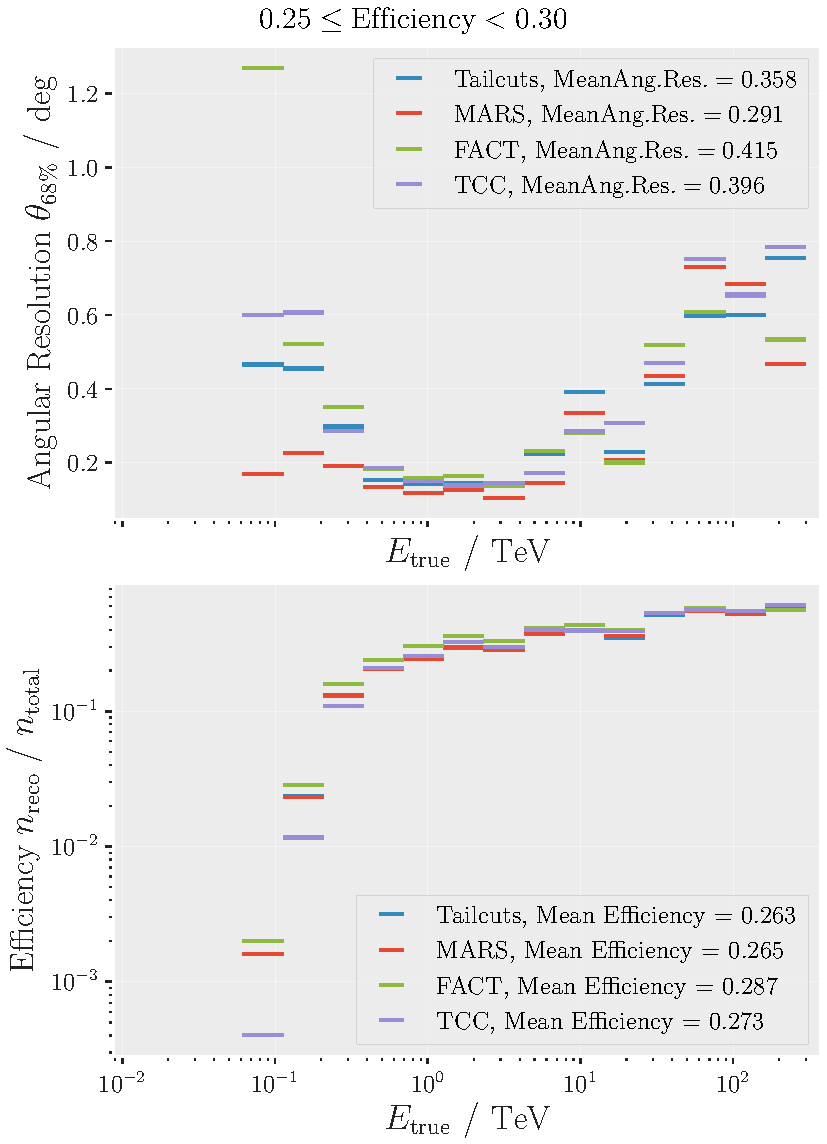
\includegraphics[width=\textwidth]{plots/ar_aeff/AR_Aeff_MST_0.25_0.30.pdf}
    \end{subfigure}
    \hfill
    \begin{subfigure}{0.45\textwidth}
        \centering
        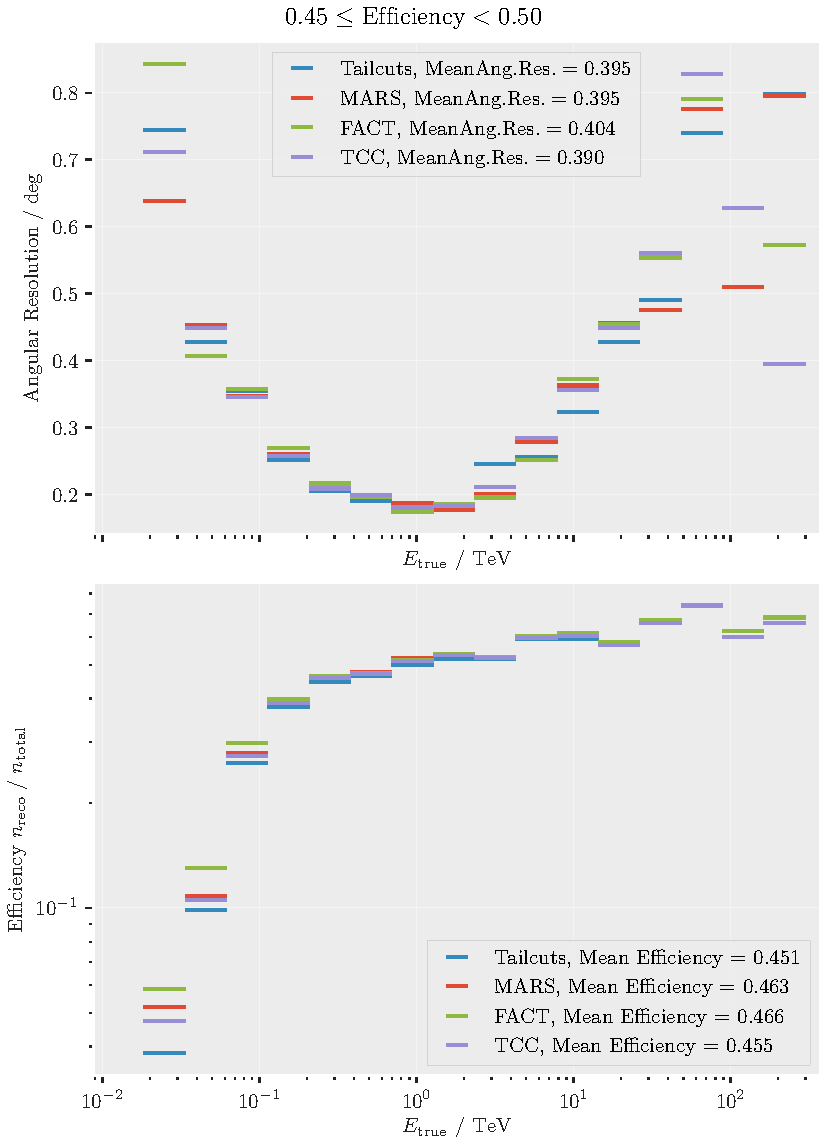
\includegraphics[width=\textwidth]{plots/ar_aeff/AR_Aeff_MST_0.45_0.50.pdf}
    \end{subfigure}
    \caption{Angular resolution and effective area for the MST simulation.}
    \label{fig:efficiency_angres}
\end{figure}

Furthermore, the mean angular resolution is plotted against the efficiency in \autoref{fig:ar_vs_eff}.

\begin{figure}
    \centering
    \includegraphics[width=0.7\textwidth]{build/ar_vs_eff.pdf}
    \caption{Angular resolution against efficiency.}
    \label{fig:ar_vs_eff}
\end{figure}

\section{Metrics of the Cleaning Algorithms}
\label{sec:metrics}




\section{Performance compared to the Default Settings}
\label{sec:performance}


\section{Comparison of the Cleaning Algorithms}
\label{sec:comparison}